%% Be sure to check spelling!

%% Put your name and the proper due date in place w/out asterisks

%% Note that two of the \lstinputlisting and 
%% all of the graphics commands are currently commented out - until the
%% files exist, processing this code without them will result in an error
%% so leave the comments until you have created the files!

\documentclass{article}
\usepackage{amsmath}    % loads AMS-Math package
\usepackage{graphicx}   % allows PostScript files
\usepackage{listings}   % allows lstlisting environment
\usepackage[letterpaper, margin=0.5in]{geometry}  % set paper size/margins
\usepackage{EGR103style}  % colorful file imports

\begin{document}
\begin{center}
\rule{6.5in}{0.5mm}\\~\\
\textbf{\large EGR 103L -- Fall 2021}\\~\\
\textbf{\huge Cantilever Starter Image}\\~\\
***NAME (NetID)***\\
***Lab Section N, DAY TIMES***\\
***DATE DUE***\\~\\
{\small I understand and have adhered to all the tenets of the Duke Community Standard in completing every part of this assignment.  I understand that a violation of any part of the Standard on any part of this assignment can result in failure of this assignment, failure of this course, and/or suspension from Duke University.} 
\rule{6.5in}{0.5mm}\\
\end{center}
\tableofcontents
\listoffigures
\pagebreak
\section{Introduction}
You do not need to change this for this assignment.

\pagebreak

\appendix
\section{Codes}
% Put the name of your file in the subsection name 
% and the listinginput input
% Be sure to include the community standard in codes!
% Add \pagebreaks if they make sense

% Note that _ in section names need \ in front (that is, \_)
% while _ in file names for lstinputlisting do not.

%%% Almost everything in this section is done; make sure you 
%%% understand how it works in general and be sure to 
%%% uncomment the lstinputlisting lines once you have created the files
\lstset{style=python103, language=python} 
\subsection{run\_can.py}
\lstinputlisting{run_can.py}

\pagebreak  % this will start figures on a new page 
\section{Figures}
%%% Almost everything in this section is done; make sure you 
%%% understand how it works in general and be sure to 
%%% uncomment the includegraphics lines once you have created the graphs
\begin{figure}[htb]
\begin{center}
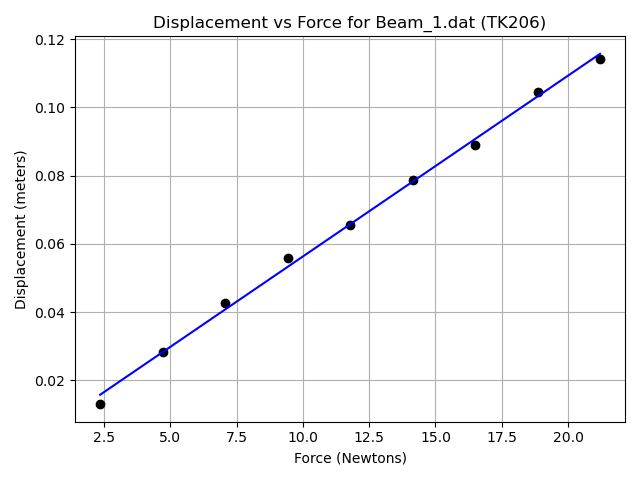
\includegraphics[width=4.5in]{RunCanPlot.png}
\caption{Displacement vs. Force for Cantilever}
\end{center}
\end{figure}

\end{document}
